\section{Towards Quantifying the Safety of Soft Robots}
In the following, we will motivate the need for a quantitative safety metric by showcasing future applications that such a metric would enable.
This will then allow us to define a list of requirements for characteristics that a safety metric needs to exhibit.
Subsequently, we contextualize the topic by reviewing the literature on how safety has been assessed and quantified in the realm of robotics before, where almost all prior work is on the safety of industrial and collaborative rigid robotic manipulators.

\begin{figure}
    \centering
    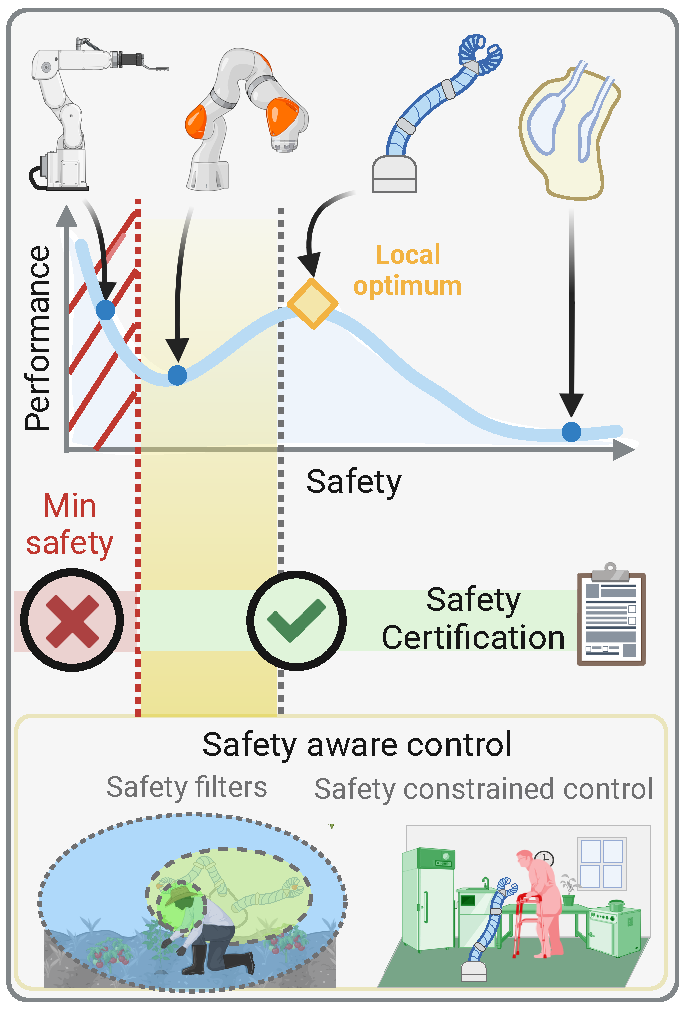
\includegraphics[width=0.5\linewidth]{safetymetric/figures/safety_metric_applications.pdf}
    \caption{Future applications that a quantitative safety metric for soft robots would enable. \textbf{Top:} Here, we showcase how the safety metric could be used for \emph{safety-aware design optimization} and, particularly, for analyzing and exploiting the performance vs. safety tradeoff. Subsequently, the safety metric could be used for certifying a given design as \emph{safe} for the respective application. \textbf{Bottom:} The safety metric could also be used for \emph{safety-aware control} - either by filtering the outputs of the controller without safety guarantees or by explicitly including the safety requirements as constraints during the optimization of the control input sequence (e.g., MPC, Control Barrier Functions).}
    \label{fig:safetymetric:safety_metric_applications}
\end{figure}

\subsection{Potential Applications for a Safety Metric}\label{sub:safetymetric:safety_metric_applications}
% We envision a safety metric for soft robots to unlock a variety of applications that we showcase in Fig.~\ref{fig:safety_metric_applications}, and that can be grouped into the domains of \emph{safety-aware control} and \emph{safety-aware design}.
We envision a safety metric for soft robots that will enable a variety of applications, as illustrated in Fig.~\ref{fig:safetymetric:safety_metric_applications}. These applications can be categorized into two main domains: \emph{safety-aware control} and \emph{safety-aware design}.

% In the domain of \emph{safety-aware control}, we assume the soft robotic design to be given, and we strive to control the actions of the soft robot in such a way that the achieved safety level remains within an acceptable range. We remark that this does not exclude contact or even collision with the environment. Instead, we strive to guarantee that these collisions do not cause any (significant) injuries. Examples include \emph{safety filters}~\cite {bertino2023prescribed} that allow us to use performant control policies that do not explicitly consider the safety constraints (e.g., RL) and still guarantee safety by filtering/saturating the control input. Alternative techniques such as MPC~\citep{hewing2020learning} or Control Barrier Functions~\citep{ames2016control}, which we refer to as \emph{safety-constrained control}, allow us to take the safety constraints directly into account when devising the control input.
In the realm of \emph{safety-aware control}, we assume the soft robotic design is already established and focus on controlling its actions to maintain an acceptable safety level. This approach does not preclude contact or collisions with the environment; rather, it ensures that such interactions do not result in significant injuries. Examples include \emph{safety filters}~\citep{bertino2023prescribed}, which allow the use of high-performance control policies (such as \gls{RL}) that do not explicitly account for safety constraints while still guaranteeing safety by filtering or saturating the control input. Alternative methods like \gls{MPC}~\citep{hewing2020learning} or Control Barrier Functions~\citep{ames2016control}—referred to as \emph{safety-constrained control}—integrate safety constraints directly into the control strategy.

% Another avenue that would be unlocked by a safety metric is \emph{safety-aware design}, which would include assessing an integrated soft robot design for its safety. Specifically, we consider here two subcategories: \emph{safety-aware design optimization} would consider safety when developing/optimizing the soft robot design either by means of inequality constraints (i.e., a minimum safety needs to be guaranteed) or by maximizing safety through the cost function.
% After a design is finalized, \emph{safety certification} would allow manufacturers to certify their product as being sufficiently safe for the respective applications (e.g., healthcare, agri-food, manufacturing, etc.). This is well-aligned with established safety standards for collaborative rigid robots as defined in ISO/TS 15066:2016~\citep{Isots_15066_2016}.
Another promising direction unlocked by a safety metric is \emph{safety-aware design}, which involves evaluating an integrated soft robot design for its safety. We see this as comprising two subcategories: \emph{safety-aware design optimization}, which incorporates safety into the design process either through inequality constraints (ensuring a minimum safety level) or by maximizing safety via the cost function; and \emph{safety certification}, where, after a design is finalized, manufacturers can certify that their product meets the necessary safety standards for specific applications (e.g., healthcare, agri-food, manufacturing, etc.). This approach aligns well with established safety standards for collaborative rigid robots as defined in ISO/TS 15066:2016~\citep{Isots_15066_2016}.

\subsection{Requirements for a Soft Robotic Safety Metric}\label{sub:safetymetric:safety_metric_requirements}
% In the following, we will list some requirements that, in our opinion, a safety metric needs to meet in order to be well suited for the applications listed in Sec.~\ref{sub:safetymetric:safety_metric_applications}.
% First (1), the metric shall consider the dynamics inherent to continuum soft robots and their particular characteristics. For example, one of the main differences between rigid and soft manipulators is that free-moving joints with integrated motors are replaced by an elastic structure that deforms under the influence of internal actuation and external forces. Therefore, any safety metric needs to crucially consider the elastic and inertial characteristics of the soft robot that are generated by the distributed material along its backbone.
% Secondly (2), the safety metric shall consider not just collision at the end-effector but instead anywhere along the body of the soft robot. This is a significant difference to the existing safety metrics for rigid/collaborative robots, which, for simplicity, usually only consider collisions at the end-effector as we would expect there the largest motion velocities~\citep{haddadin2011safe, Isots_15066_2016}. Instead, soft robots exhibit large Cartesian stiffnesses close to their proximal end, thus requiring us to consider the safety of collisions anywhere along the backbone.
% Next, (3) any simplifying assumptions shall lead to a conservative estimate of the achieved safety. For example, soft robot models underlying the safety metric would likely use a finite-dimensional approximation of the continuum shape; instead, in reality, flexible structures such as soft robots exhibit infinite degrees of freedom~\citep{della2023model, armanini2023soft}. Therefore, we would like any safety metric making use of finite-dimensional approximations to underestimate instead of overestimate the safety of the design.
% Fourthly (4), the computation of the safety metric shall be computationally tractable, which is essential for safety-aware control and design applications, where evaluations on the scale of sub-seconds and seconds are necessary.
% Finally, we end with a few desirable characteristics: (5) some applications, such as safety-aware control or safety-aware design, might benefit from the differentiability of the safety metric with respect to design parameters, robot states, and control inputs; (6) ideally, the safety metric shall also consider how \emph{safe} the soft robot's design (e.g., friendly-looking) and behavior (e.g., smooth and predictable movements) is perceived by the user. In addition to user studies, the evaluation of this metric might be assisted by VLMs.
In the following, we outline several requirements that, in our opinion, a safety metric must satisfy to be well-suited for the applications described in Sec.~\ref{sub:safetymetric:safety_metric_applications}. First (1), the metric should account for the dynamics inherent to continuum soft robots and their unique characteristics. For example, a primary difference between rigid and soft manipulators is that free-moving joints with integrated motors are replaced by a compliant structure that deforms under internal actuation and external forces. Consequently, any safety metric must consider the elastic and inertial properties generated by the distributed material along the robot’s backbone.
%
Secondly (2), the safety metric must evaluate collisions occurring anywhere along the soft robot’s body—not just at the end-effector. This represents a significant departure from existing safety metrics for rigid or collaborative robots, which often focus solely on the end-effector due to its typically higher motion velocities~\citep{haddadin2009requirements, haddadin2011safe, Isots_15066_2016}. In contrast, soft robots exhibit high Cartesian stiffness near their proximal end, making it necessary to assess safety along the entire structure.
% 
Next (3), any simplifying assumptions should yield a conservative safety estimate. For instance, while soft robot models used in the metric might employ a finite-dimensional approximation of the continuum shape, in reality, these flexible structures possess infinite degrees of freedom~\citep{della2023model, armanini2023soft}. Therefore, a safety metric based on such approximations should tend to underestimate rather than overestimate the design’s safety.
% 
Fourthly (4), the computation of the safety metric must be tractable, which is essential for safety-aware control and design applications that require evaluations on sub-second to second timescales, respectively.
% 
Finally, we highlight a few desirable characteristics: (5) in applications such as safety-aware control or design, it is advantageous if the safety metric is differentiable with respect to design parameters, robot states, and control inputs; and (6) ideally, the metric should also reflect how “safe” the soft robot’s design (e.g., its friendly appearance) and behavior (e.g., smooth and predictable movements) are perceived by users. In addition to user studies, the evaluation of this metric might be enhanced by leveraging \glspl{VLM}~\citep{touvron2023llama, grattafiori2024llama}.

\subsection{Background on Injury Risk Criteria for Robotic Manipulators}

\begin{itemize}
    \item Give a motivation for why the robotics community strives to quantify safety/injury risk (e.g., optimizing designs and controllers to make them more human-friendly, safety-aware control, etc.).
    \item Give an overview of the trailblazing literature on measuring the injury risk of rigid robots.
    \item Mention the ISO norm that establishes the standards for safe, collaborative robots.
    \item List the existing attempts to assess the safety of soft robots and why they are not sufficient (e.g., too simplistic models, not taking into account the control, lacking a contact model, etc.)
    \item List some of the initial attempts to give designers an idea of which factors influence the safety of soft robots (e.g.,~\citep{abidi2017intrinsic}).
\end{itemize}

\textcolor{red}{Stucture: \begin{enumerate}
    \item Motivation for measuring safety: selecting suitable design, defining constraints that guarantee safety (i.e., ISO norms), and safety-aware control and motion planning
    \item Stress that this is a well-established line of research in (rigid) robotics involving both conceptual and experimental analysis
    \item Modes of impact and injury: constrained vs. unconstrained (human), static vs. dynamic, sharp surfaces, different body parts, etc.~\citep{haddadin2009requirements}
    \item Injurity severity criterias: the first were based on automobile crash models (HIC), but found to be unsuitable as they are calibrated for higher velocities and inertias that are not even relevant for rigid robots. In particular, taking the head acceleration as a injury criteria is not suitable, as not in practice reached, even when robots are moving at 2m/s. Furthermore, it mostly focuses on the question of fatale impacts. Instead, other injury modes, even if not fatal, become relevant as (rigid) robots can still cause bones to break and other significant injuries at their speeds. There exist specialized injury severity criteria inspired by biomechanics for the various body parts. For example, body parts have different contact stiffnesses and injury is (most likely) caused when different thresholds are exceeded (e.g., penetration depth, maximum force, energy density, acceleration). However, it seems that most of them are correlated with the the maximum force experienced during impact and that the maximum force generalizes the best across body parts.
    \item Mention ISO/TS 15066:2016 (Collaborative robots) and ISO/PAS 5672:2023
    \item Safety metrics for soft robots: basically not existing, only~\citep{abidi2017intrinsic}, but only super-simplified beam model. A safety metric is especially important for soft robots as we continuously stress the inherent safety of soft robots, so we also need to be able to quantify it.
\end{enumerate}}

Various aspects have motivated the robotic community to try to assess the safety of our robots~\citep{de2008atlas, van2018spatial}: 
First of all, understanding the important factors influencing safety allows us to make robotic designs and control algorithms safer~\citep{bicchi2004fast, zinn2004new}. 
Secondly, quantifying the injury risk stemming from a robot allows the establishment of minimal safety standards and specifically constraints on the design and actuation that guarantee safe deployment of the robots, as done, for example, in ISO 10218-1:2011~\citep{iso2011robots} for industrial robots and ISO/TS 15066:2016~\citep{Isots_15066_2016} for collaborative robots. This allows the designers and manufacturers of robots to certify that their design is \emph{safe}, which is, in turn, crucial for successful adoption by industrial customers and consumers.
Thirdly, modeling the injury risk of robots and explicitly setting operation constraints that guarantee safety enables safety-aware control~\citep{lacevic2011safety, zanchettin2015safety, mansfeld2018safety}, motion planning~\citep{lacevic2022safe, pupa2024efficient} and also the deployment of safety filters~\citep{hewing2020learning, bertino2023prescribed}.

% Before improving the safety of (collaborative) robots, we first need to understand the important factors influencing the injury risk and be able to compare different robot design w.r.t. to their achieved safety level~\citep{de2008atlas}.
For the reasons mentioned above, quantifying the safety and associated injury risk has been a longstanding research topic, with most effort centered on determining the safety of collaborative rigid robotic manipulators~\citep{zinn2004playing, bicchi2004fast, haddadin2009requirements, mansfeld2018safety}.